\section{State of the Art}
\label{section:state-of-the-art}

This section addresses some of the important state of the art in MDE approaches to BX, focusing on three specific elements: important BX \textit{scenarios} that have been identified in the literature; important \textit{languages} that have been influential in research in BX -- in this case, we focus on QVT; and important \textit{tools} that implement aspects of BX and that are based on MDE technology. We do not consider non-MDE approaches to BX in this brief review, and we also exclude TGG approaches because these are covered in detail by other lectures.

\subsection{BX Scenarios}
A number of recurring scenarios of use for BX have appeared in the MDE literature. Many of the MDE tools and languages that we discuss in the sequel have been designed to address these scenarios.

\begin{enumerate}
\item \textit{Round-trip engineering}, i.e., generating code from models, modifying the code by hand, and then regenerating the models to reflect changes made in the code. A BX approach would, conceptually, aim to apply the principle of least change and minimise the number of modifications necessary to the original model, instead of regenerating the entire model after each change. Research in MDE related to incremental transformation is also addressing this scenario.

\item \textit{Collaborative modelling}, wherein multiple stakeholders are editing the same model simultaneously. In practice, what often happens is that each stakeholder has a local copy (or view) of the source model, and their changes are reflected back on the master/source copy at specified points of time.

\item \textit{Synchronisation,} e.g., synchronising documents and code, like assurance cases and source code. This is related to round-trip engineering but synchronisation can involve model management operations other than transformations.

\item \textit{Reflection,} for example, reflecting the results of some kind of analysis in a source model. A concrete instance of this was investigated in the MADES project where a UML MARTE model was transformed into a variety of formal models (UPPAAL, TRIO) to support analysis, and some of the results of the analysis were reflected in the MARTE models. This is an interesting example of a BX as the backwards transformation is generating a view of the target model which needs to be synchronised with the source model.
\end{enumerate}

\subsection{Standard MDE languages for BX: QVT}
While there are numerous tools and approaches, based on MDE technology (like Eclipse EMF) for supporting BX, most of these approaches are strongly influenced by a significant standardised language for transformation: the OMG's Query, View and Transformations (QVT) standard \cite{QVT-specification}. QVT is a family of languages that were first envisaged in 2002 upon issue of an OMG request for proposals to support aspects of the OMG's Model-Driven Architecture standard. A number of replies were received, and the first version was submitted and approved in 2005. The most recent version, QVT 1.3, was released in June 2016. 

QVT, as mentioned, is a family of languages. These languages are meant to support transformation and querying of MOF models; transformations and queries in turn can be used to generate views. The basic architecture of QVT is illustrated in Figure~\ref{fig:qvt}. The QVT architecture builds on other OMG languages, particularly MOF but also the Object Constraint Language (OCL), from which QVT acquires its expression and collection manipulation facilities.

\begin{figure}[htbp]
\centering{\scalebox{0.6}{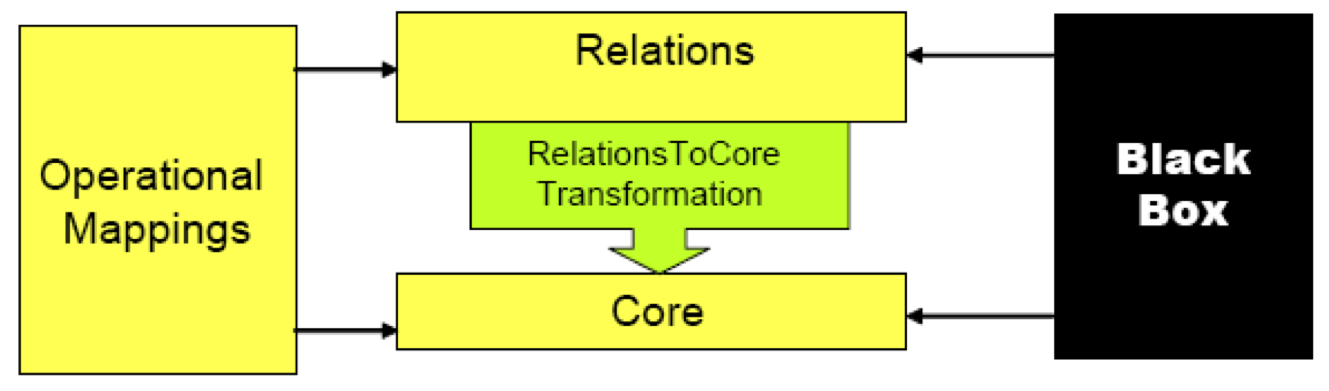
\includegraphics{qvt-architecture.png}}}
\label{fig:qvt}
\caption{QVT architecture from \cite{qvt}}
\end{figure}

The Relations language provides mechanisms for the declarative specification of the relationships between MOF models. It in turn supports complex object pattern matching, and implicitly creates trace classes and their instances to record what occurred during the execution of a transformation. Assertions can also be made; for instance, relations can assert that other relations also hold between particular model elements matched by their patterns. As illustrated in the figure, the intention is that Relations specifications can be translated in to the QVT Core language, along with a set of trace models, which in total provide a formal semantics for QVT Relations.

QVT Core, by contrast, is a small yet expressive language that only supports pattern matching over a flat set of variables by evaluating conditions
over those variables against a set of models. It is intended to be semantically equivalent to QVT Relations, but equivalent QVT Relations programs are liable to be more concise than the QVT Core programs.

The Operational Mappings (sometimes called QVT Operations, or QVT-o) is an operational model transformation language that extends Relations with imperative constructs. Of all the QVT languages, it is QVT-o that has received the most use and attention.

The abstract syntax of the Relations language is illustrated in Figure~\ref{fig:qvt-as}.

\begin{figure}[htbp]
\centering{\scalebox{0.6}{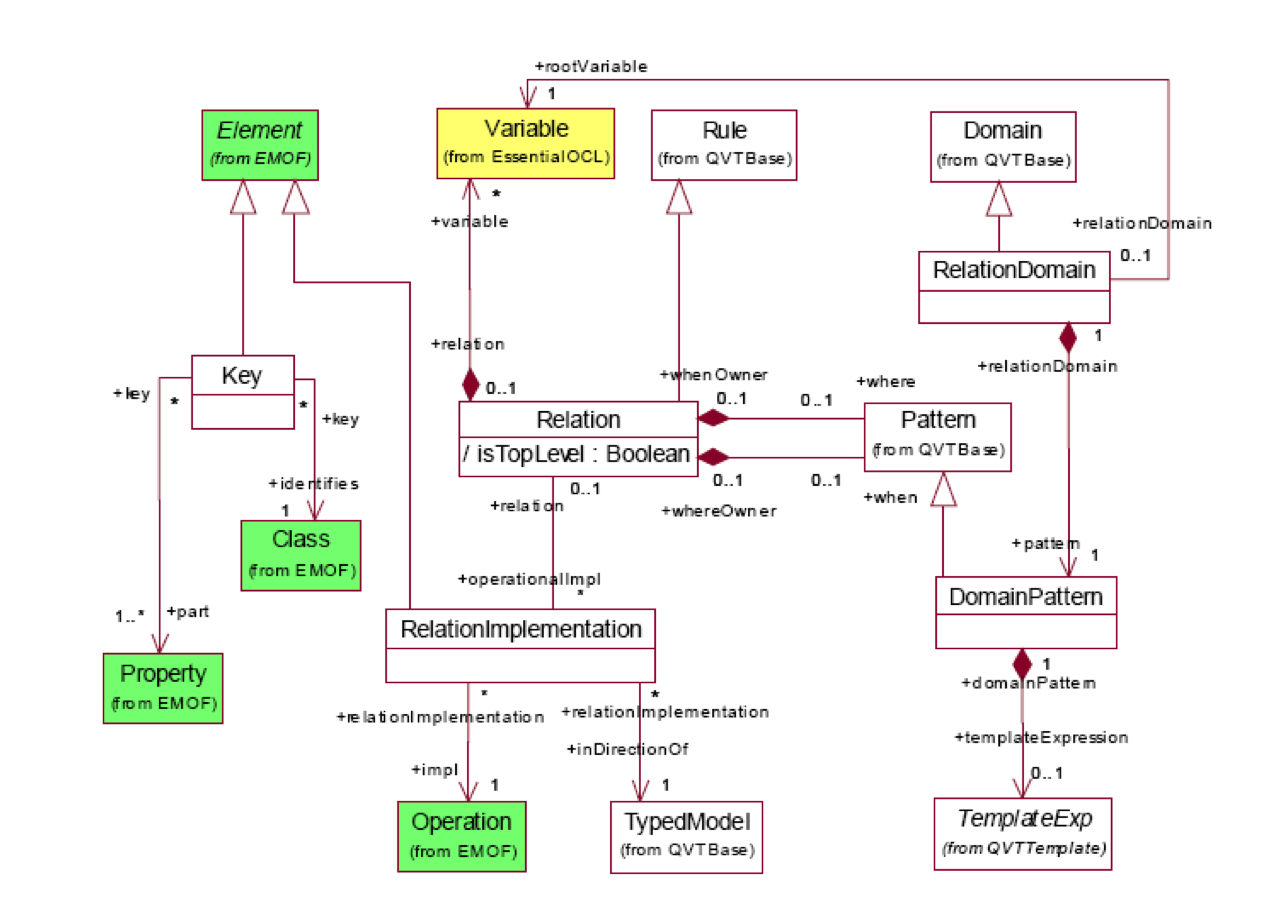
\includegraphics{qvt-relations-metamodel.png}}}
\label{fig:qvt-as}
\caption{QVT Relations abstract syntax}
\end{figure}

The abstract syntax can be interpreted as follows: a QVT Relations program contains a set of rules which are relations. Relations are made up of a patterns, and are applied to a set of typed model parameters. In particular, these relations can be interpreted in forward and backwards directions -- that is, Relations is a BX by design.

An example of the concrete syntax of Relations is shown in Listing~\ref{listing:qvt-relations}. This example gives a relation that is used to map persistent classes in an object oriented program to a table. The example includes three parts: a domain (a set of patterns which defines the variables and constraints that model elements bound to those variables must satisfy -- i.e., the bindings for the relation); the \textit{when} clause (the conditions under which the relation must hold); and the \textit{where} clause (the condition that must be satisfied by all model elements participating in the relation). The interpretation of when-clauses in the Eclipse QVT implementation is that these are preconditions, and where-clause are postconditions. Both of these clauses may contain arbitrary OCL expressions.

\begin{lstlisting}[caption=An example of QVT Relations, label=listing:qvt-relations]
relation ClassToTable /* map persistent class to table */
{
  domain uml c:Class {
      namespace = p:Package {},
      kind = 'Persistent',
      name = cn
  }
  domain rdbms t: Table {
      schema = s:Schema {},
      name = cn,
      column = cl:Column {
        name = cn + '_tid',
        type = 'NUMBER'},
        primaryKey = k:PrimaryKey {
          name = cn + '_pk',
          column = cl }
   }
   when { 
     PackageToSchema(p,s);
   }
   where {
      AttributeToColumn(c,t);
    }
}
\end{lstlisting}
In this particular example, the domain clauses establish which model elements in a UML and a RDBMS model are of interest (they satisfy the predicate part of the domain clauses), and the when and where clauses are defined elsewhere by other relations.

The BX capabilities of QVT can also be illustrated by an example from QVT Core. Figure~\ref{fig:qvt-core} illustrates an example of a single mapping rule in QVT Core. This is a \textit{checking} example, which is used to check that particular patterns are satisfied by models. Once again, this is an example involving relations between a UML class model and a database model. The top part of the diagram (labelled Class to Table) defines the \textit{c2t} relation, which relates a class to a table. The bottom pattern is evaluated using variable values of a valid binding (a valid pair of class and table) from the top pattern. In effect, the top part of the mapping rule defines a guard which restricts the scope of the bottom part of the rule.

\begin{figure}[htbp]
\centering{\scalebox{0.5}{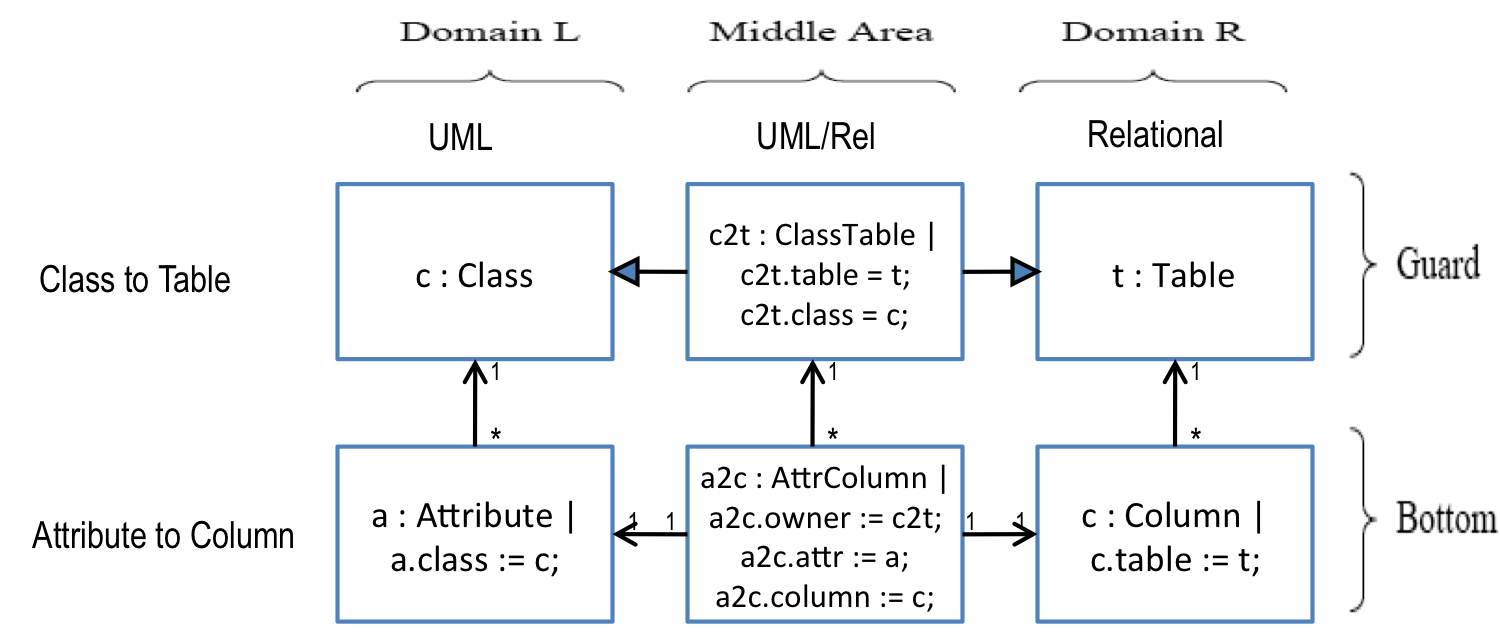
\includegraphics{mapping-rule.png}}}
\label{fig:qvt-core}
\caption{QVT Core: mapping rule example}
\end{figure}

Once again, the mapping rule is directionless; it can be executed either way, checking a database table against a UML class, or vice versa.

The QVT standard is currently being further developed, both through the OMG standardisation efforts, but also through work on Eclipse QVT, an implementation of the different QVT languages. We briefly discuss the status of Eclipse QVT, and other MDE tools for BX, in the next subsection.

\subsection{Tools}
In this section we briefly outline some of the key tools, based on MDE technologies and principles, that either support or claim to support BX. As mentioned earlier, we exclude approaches based on triple graph grammars as these are covered elsewhere.

\subsubsection{Medini}
Medini\footnote{\url{http://projects.ikv.de/qvt/wiki}} claims to be a reasonably complete implementation of QVT Relations, but is currently unsupported. It is an EMF based transformation engine but also has a non-commercial licensed editor and debugger. While it uses the the QVT Relations syntax, it intentionally departs from the semantics of the OMG standard (e.g., how it supports deletion of elements, that it does not provide a checkonly mode). As such, we prefer not to label Medini as an implementation of QVT.

\subsubsection{ModelMorf}
ModelMorf is a proprietary tool from Tata Consulting Services\footnote{Archived copy available at \url{https://web.archive.org/web/20120323171429/http://www.tcs-trddc.com/trddc_website/ModelMorf/ModelMorf.htm}}. It also claims to faithfully implement the QVT Relations standard, but research by Stevens \cite{Stevens13} shows that it does not fully implement the semantics specified in the standard. By some measures, it is more faithful than Medini, but it is still not a full implementation of QVT.

\subsubsection{jQVT}
jQVT\footnote{\url{https://sourceforge.net/projects/jqvt/}} is a QVT-like engine that is defined on top of the Java type system instead of using EMF. In turn, it uses Xbase (a partial programming language written in Xtext which compiles to Java and includes powerful features such as closures) instead of OCL for expressions. In essence, jQVT is a Java embedding of QVT; the jQVT engine generates native Java code from jQVT scripts. Of note is that it does provide support for bidirectional transformations. As of early 2016 jQVT was still being maintained.

\subsubsection{Echo}
Echo\footnote{\url{http://haslab.github.io/echo/}} is an open-source EMF-based tool for model repair and transformation that exploits the Alloy model finder to determine models that satisfy relations. It in turn provides an implementation of the QVT Relations syntax, but the semantics intentionally departs from the OMG specification. Echo is also bidirectional.

\subsubsection{JTL}
The Janus Transformation Language (JTL)\footnote{\url{http://jtl.di.univaq.it/}} is a by-design bidirectional language with a QVT-like syntax, which propagates changes made in one model to the other. If a change made to one model makes the second model inconsistent, an approximation (``closest match'') is calculated using answer set programming. As such, there can be several solutions to a transformation problem and the results provided by JTL may need to be constrained further.

\subsubsection{Eclipse QVT}
Substantial engineering effort is being put into the development of Eclipse QVT, a project that
aims to support the full OMG QVT specification (though with Ecore instead of MOF models). Currently, QVT Operations is well supported and active as part of the Eclipse M2M project. QVT Relations (in Eclipse terms, QVT Declarative) and QVT Core are work-in-progress. As work on these projects is ongoing and their status is changing regularly, we refer the reader to the Eclipse MMT project website\footnote{\url{https://projects.eclipse.org/projects/modeling.mmt}} for the latest information. As of this writing, the intention with Eclipse QVT is that the Oxygen release in June 2017 will provide full support for QVT Relations.

\subsubsection{Bidirectionalisation}
There have been several approaches to so-called \textit{bidirectionalisation} of transformations. In these approaches, a forward transformation (from source to target) is written and the backward transformation is calculated or computed automatically. Examples of this approach include that of Hoisl \cite{HoislHH14a}. The GRoundTram approach of Sasano is another example \cite{SasanoHHIKN11}.

\vspace{4mm}

For further details, and a more in-depth classification of MDE approaches to BX, the interested reader is referred to Hidaka et al's excellent survey of BX \cite{HidakaTCH16}.


